\section{Evaluation}~\label{sec:eval}
Our evaluation focuses on the effectiveness  and scalability of our approach.
To measure the effectiveness, we compare with the predictive analysis, {\sf RV}~\cite{}. We choose RV for two main reasons: (1) {\sf RV} is the only open source predictive analysis, (2) {\sf RV} represents the state-of-the-art approach, which is theoretically proven to have higher detection capability than other approaches. 

{\bf Evaluation Method} We conduct our experiment on a large set of applications, which are also used to evaluate {\sf RV}. Specifically, the set includes large applications such as {\sf Jigsaw}, {\sf Xalan}, {\sf Lusearch}. For the large applications that use the reflection, we adopt {\sf Tamiflex}~\cite{} to 
to support the static analysis, which replaces the reflection calls with the concrete method calls recorded in the observation run.  We omit the benchmark {\sf eclipse} because the current version of {\sf Tamiflex}  leads to abnormal execution after the instrumentation, which throws exception during starting the main service. By applying our tool to such abnormal execution, we identify only 3 races, similar to the report of RV~\cite{}.
Besides, the benchmark {\sf montecarlo} requires the input, which we downloaded from internet and simplified. For the large applications, we use the most lightweight configuration if possible.


 As the detection capability  depends on the observed run, for fair comparison, we monitor the execution once by recording all necessary information required by both approaches, and then apply both techniques to the monitored run. Besides, our reported data for RV may be different from the original report for two reasons: (1) the different observed runs lead to different set of races, (2) the original implementation of RV contains a bug in identification of the branches, which leads to the misses of many branches and the incorrect reduction of dependences during the analysis. We confirmed the bug with the author and fixed the bug in our experiments~\footnote{We report the bug in details with the test case \url{https://sites.google.com/site/recipe3141/}}.  


Our experiments and measurements 
were all conducted on an x86 64 Thinkpad W530 worksta- 
tion with eight 2.30GHz Intel Core i7-3610QM processors, 
16GB of RAM and 6M caches. The workstation runs version 12.04 of the Ubuntu Linux distribution, and has the Sun 
64-Bit 1.6.0\_26 Java virtual machine (JVM) installed~\footnote{Note that Sun JDK 1.7 does not support the transformation of dacapo applications with {\sf tamiflex}.}. 


%Specifically, we use two threads in the monitored run as two threads are sufficient to manifest most of races~\cite{shanlu}. 








\subsection{Effectiveness}
Table~\ref{tab:main} shows the main results of our analysis, which includes four sections: Trace (details about the trace), Races (detected races), Difference (comparison with RV) and Running time (the time taken by the analysis).


The Trace section includes the number of threads ($Th$), the number of shared reads ($Reads$) and shared writes ($Writes$), the subset of shared reads that read the base object references  ($Base$), where the  base object references are references used as the base/target in the following field reference or the method invocation,  the number of branches ($Br$), the synchronization events ($Sync$) and the total number of events ($Total$), which includes local accesses in addition to the aforementioned events. Specifically, for the branch, we report it in the form of $A/B$, where $A$ refers to the number of branches used by our analysis and $B$ refers to the number of branches used by RV. To ensure that the predicted run sees the same base object at each shared read/write, {\sf RV} inserts the artificial branch immediately in front of each shared access (and array accesses). We do not use such artificial branches.


We make interesting observations about the Trace section. The non-local events, i.e., all the events listed in Table~\ref{tab:main}, occupy around 30\% of the total trace in the first 7 benchmarks, but occupy less than 1\% of the trace in the rest benchmarks, which have relatively more complex logic. The reads of the shared base objects occupy a small portion ($1/3$-$1/10$) of the total shared reads. The rest shared reads read only the primitive values or 
the references that are not the base references, e.g., the references involved only in the nullness check. Besides, our analysis involves significantly less branch events as compared to the {\sf RV} approach. The difference plays an important role in the detection, which we will explain shortly.


The $Races$ section shows the number of races detected by {\sf Recipe-s}, i.e., {\sf Recipe} without exploring un-executed paths, {\sf Recipe}, i.e., the fully-fledged version, and {\sf RV}. By comparing the {\sf Recipe-s} and {\sf Recipe}, we find {\sf Recipe} finds 100+ more races, which demonstrates the strength of exploring  un-executed paths. Intuitively,  {\sf Recipe-s} predicts based on a single trace, while {\sf Recipe} predicts based on multiple traces containing different execution paths. We also compare the {\sf Recipe} version with {\sf RV} version, as illustrated in the $Difference$ section, where $Diff$ shows the races found by {\sf Recipe} but missed by {\sf RV}, $Diff'$ shows the races found by {\sf RV} but missed by {\sf Recipe}.

First of all, {\sf Recipe} finds many 150+ more races than {\sf RV}. The reasons are multifold: (1) {\sf Recipe} can reason about the accesses in the un-executed paths, while {\sf RV} and {\sf Recipe-s} can only reason about the accesses in the executed paths. (2) {\sf Recipe} or {\sf Recipe-s} allows the relaxation of the scheduling even if it breaks the inter-thread read/write dependence in the observed run. {\sf Recipe} allows the majority of the shared reads, i.e., the reads of primitive values, to freely read from a different value from a different write as long as the value leads to the same branch decisions. {\sf RV}, however, requires them to read the same values as in the observed run. (3) An critical optimization proposed by {\sf RV} is to preserve dependences only for the reads before the preceding branches  of the racy events, rather than all the reads. However, this optimization is underplayed by the fact that {\sf RV} introduces huge amount of artificial branches, i.e., one before each shared field access, which ensures the use of the same base objects.
We get rid of such artificial branches and instead, rely on the small amount of base read events to ensure the use of the same base objects (Section~\ref{}). Our strategy reduces the number of branches greatly and amplifies the effectiveness of the optimization. We also conduct case studies (Section~\ref{}) to better illustrate the scenarios.

 

Another interesting observation is, although {\sf Recipe} should produce all races found by {\sf RV} in theory, {\sf Recipe} may miss races found by {\sf RV} in practice (Column $Diff'$), i.e., {\sf Recipe} is not strictly more effective than {\sf RV} in practice. The underlying reason is due to the limits of the constraint solver: (1) the solver cannot compute constraints with very complex arithmatic operations (2) the solver does not support some program constants such as the scientific notation, $3E-10$.

The last section, Running time, compares the analysis time for both approaches. We find our approach is significantly slower than {\sf RV}, e.g., {\sf RV} often finishes within 200 seconds, while our approach may take more than 1 hour. This is because our approach needs to reason about the computation among variables inside the local access events, while {\sf RV} needs to only reason about the order relations among the events.

{\bf Summary of advantage and weakness\ } In general, our approach is flexible, which allows the relaxation of schedules and paths based on the fine-grained reasoning of value flows. As a result, it detects many more races compared to existing approaches. On the other hand, it is heavy weighted. The suggestion is to combine it with the lightweight approach with soundness guarantee such as {\sf RV}, by treating {\sf RV} as the preprocessing and instructing {\sf Recipe} to skip those confirmed by {\sf RV}. In this way, we can complement {\sf Recipe} by finding those missed by it due to the limit of the constraint solver.
 











%TODO Reorder the columns: RV ReceipeS Recipe


\begin{table*}[htbp]
\caption{Relaxed Analysis}
\begin{flushleft}
\begin{tabular}{|l|r|r|r|r|l|r|r|r|r|r|r|r|r|r|}
\hline
 & \multicolumn{ 7}{c|}{Trace} & \multicolumn{ 3}{c|}{Races} & \multicolumn{ 2}{c|}{Difference} & \multicolumn{ 2}{c|}{Running time (sec)} \\ \hline
Benchmarks & \multicolumn{1}{l|}{Th} & \multicolumn{1}{l|}{Reads} & \multicolumn{1}{l|}{Writes} & \multicolumn{1}{l|}{Base} & Br & \multicolumn{1}{l|}{sync} & \multicolumn{1}{l|}{Total} & \multicolumn{1}{l|}{Recipe-s} & \multicolumn{1}{l|}{Recipe} & \multicolumn{1}{l|}{RV} & \multicolumn{1}{l|}{Diff} & \multicolumn{1}{l|}{Diff'} & \multicolumn{1}{l|}{Recipe} & \multicolumn{1}{l|}{RV} \\ \hline
critical & 3 & 13 & 7 & 5 & 2/13 & 6 & 78 & 8 & 8 & 8 & \multicolumn{1}{c|}{0} & 0 & 8 & \multicolumn{1}{c|}{2} \\ \hline
airline & 11 & 45 & 15 & 4 & 32/82 & 30 & 317 & 9 & 9 & 9 & 0 & 0 & 490 & 4 \\ \hline
account & 3 & 46 & 21 & 10 & 3/47 & 6 & 227 & 2 & 5 & 5 & 3 & 3 & 41 & 4 \\ \hline
pingpong & 4 & 7 & 7 & 3 & 0/15 & 6 & 111 & 1 & 1 & 1 & 0 & 0 & 19 & 1 \\ \hline
bbuffer & 4 & 640 & 118 & 10 & 634/1.1K & 217 & 3.3K & 13 & 25 & 9 & 21 & 5 & 62 & 5 \\ \hline
bubblesort & 26 & 1.3k & 966 & 121 & 155/2.8K & 322 & 8.4K & 7 & 7 & 7 & 0 & 0 & 3295 & 3 \\ \hline
bufwriter & 5 & 165 & 52 & 75 & 16/130 & 44 & 525 & 4 & 10 & 2 & 8 & 0 & 63 & 9 \\ \hline
mergesort & 5 & 38 & 33 & 5 & 15/472 & 28 & 1.7K & 3 & 10 & 3 & 10 & 0 & 37 & 5 \\ \hline
raytracer & 2 & 31 & 5 & 12 & 314/8,2K & 676 & 94.5K & 4 & 6 & 4 & 2 & 0 & 47 & 2 \\ \hline
montecarlo & 2 & 5 & 86 & 2 & 1.9K/38.2K & 21.1K & 1.9M & 1 & 4 & 1 & 3 & 0 & 1 & 17 \\ \hline
moldyn & 2 & 605 & 61 & 104 & 19.6K/52.6K & 62 & 203.4K & 6 & 14 & 2 & 12 & 0 & 2842 & 1 \\ \hline
ftpserver & 28 & 684 & 299 & 71 & 4.4K/233.3K & 78.2K & 3.9M & 99 & 152 & 57 & 108 & 13 & 811 & 153 \\ \hline
jigsaw & 12 & 525 & 702 & 211 & 63.2K/467.9K & 86.7K & 5.5M & 17 & 23 & 8 & 15 & 0 & 33 & 7 \\ \hline
sunflow & 9 & \multicolumn{1}{l|}{2.1K} & \multicolumn{1}{l|}{1.3K} & 473 & 201.3K/827.0K & 50K & \multicolumn{1}{l|}{7.1M} & 38 & 78 & 20 & 69 & 11 & 4520 & 22 \\ \hline
xalan & 9 & \multicolumn{1}{l|}{1.4K} & \multicolumn{1}{l|}{0.9K} & 209 & 15.7K/103.2K & \multicolumn{1}{l|}{190.1K} & \multicolumn{1}{l|}{6.6M} & 2 & 6 & 2 & 4 & 0 & 5317 & 10 \\ \hline
lusearch & 10 & \multicolumn{1}{l|}{2.3K} & \multicolumn{1}{l|}{0.5K} & 715 & 22.2K/164K & \multicolumn{1}{l|}{93.2K} & \multicolumn{1}{l|}{9.1M} & 27 & 49 & 14 & 38 & 5 & 5430 & 8 \\ \hline
\end{tabular}
\end{flushleft}
\label{tab:main}
\end{table*}









  



\subsection{Case studies}
We manually inspect the reported races in small applications to gain better understanding about our approach. 

{\bf Relaxing the Inter-thread dependence\ } Figure~\ref{fig:relax1} demonstrates the relaxation of inter-thread dependence enabled by our approach. 
The code is from the benchmark {\sf bbuffer}, where the line number is marked. Huang et al.~\cite{} detects the race between line 291 and line 400, but fails to detect the race between line 294 and line 400. The reason is as follows. In the observation run, the execution follows the order,  lines 400, 291 and 294. For the event at line 294, its preceding branch at line 291 reads from line 400. Therefore, Huang et al.~\cite{}
 requires the predicted run to preserve the dependence between line 291 and line 400 so that line 291 reads exactly the same value and the branch takes the same branch decision. The dependence enforces the order constraint, $400 \rightarrow 291$, which further enforces the order $400\rightarrow 291 \rightarrow 294$.    Our approach does not require the existence of such dependence. Specifically, we allow line 291 to happen before line 400 in the predicted run as long as the value read by it leads to the same branch decision, which is true in this case.  As a result, there is no order constraint between line 294 and line 400, and the two forms a race. We re-replay such race  easily using the eclipse IDE breakpoints. 


 

\begin{figure}[htp]
\centering
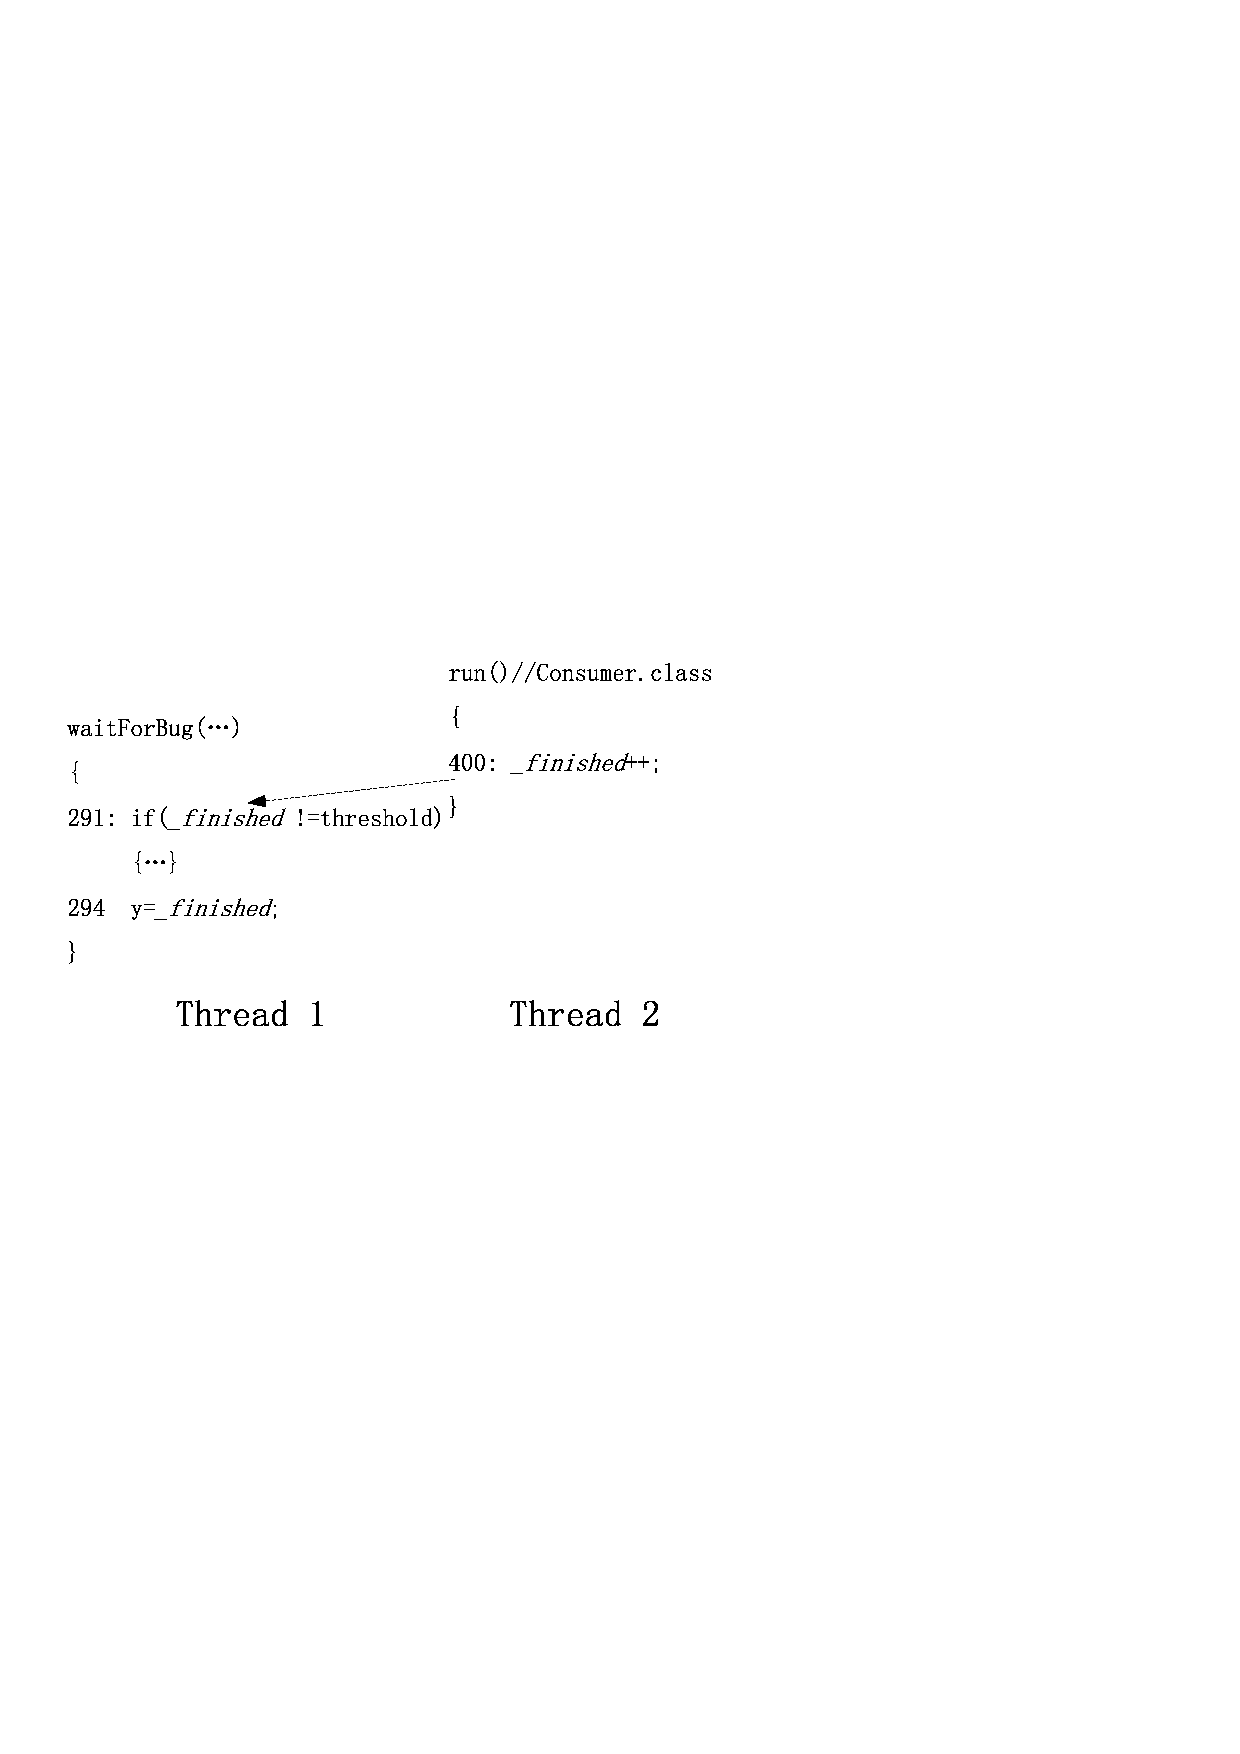
\includegraphics[scale=0.7]{cases/Visio-bbuffer.pdf}
\caption{Relaxation of Inter-thread dependence}\label{fig:relax1}
\end{figure}

{\bf Relaxing the Paths\ } Figure~\ref{fig:relax2} demonstrates how our approach relaxes the schedulings to account for the unexecuted paths. 
Each thread invokes the method {\sf Sorting}, which recursively starts two children threads if there are two more available entries in the thread pool (lines 8-11), or  starts one child thread if there is only one available entry (lines 4-5).  The availability is computed through the static method {\sf available} with the constant {\tt total}, which is equal to 5. The shared variable {\tt alive} denotes the used entries.

 
Initially there is one sorting thread. After it starts Thread 1 and Thread 2, there are three threads alive and only two more entries are available.
Suppose in the observation run, Thread 2 consumes both thread entries and starts the children Thread 3 and Thread 4 (not shown), updating {\tt alive} to 5, then Thread 1 cannot execute the branch at lines 4-5. Huang et al.~\cite{} require the predicted run to preserve the dependence denoted by the dotted line since the dependence affects the branch condition at line 2. As a result, the predicted run follows the same branch decision and cannot reason about the code at lines 4-5. Our analysis does not have such limitation. Instead, it allows the predicted run to reason about the un-explored code. Specifically, it does not need to preserve the dependence from line 11 to line 1 and it allows line 1 (Thread 1) to read from line 9 (Thread 2). As a result, the branch condition guarding the unexplored branch is evaluated to be true, enabling the unexplored path in the constraint solver. Finally, the solver identifies the race between line 5 (Thread 1) and line 1 (Thread 3). Note that the two lines are synchronized on different locks~\footnote{We abbreviate the {\tt synchronized} keyword as {\tt sync}.
}. 

 


\begin{figure}[htp]
\centering
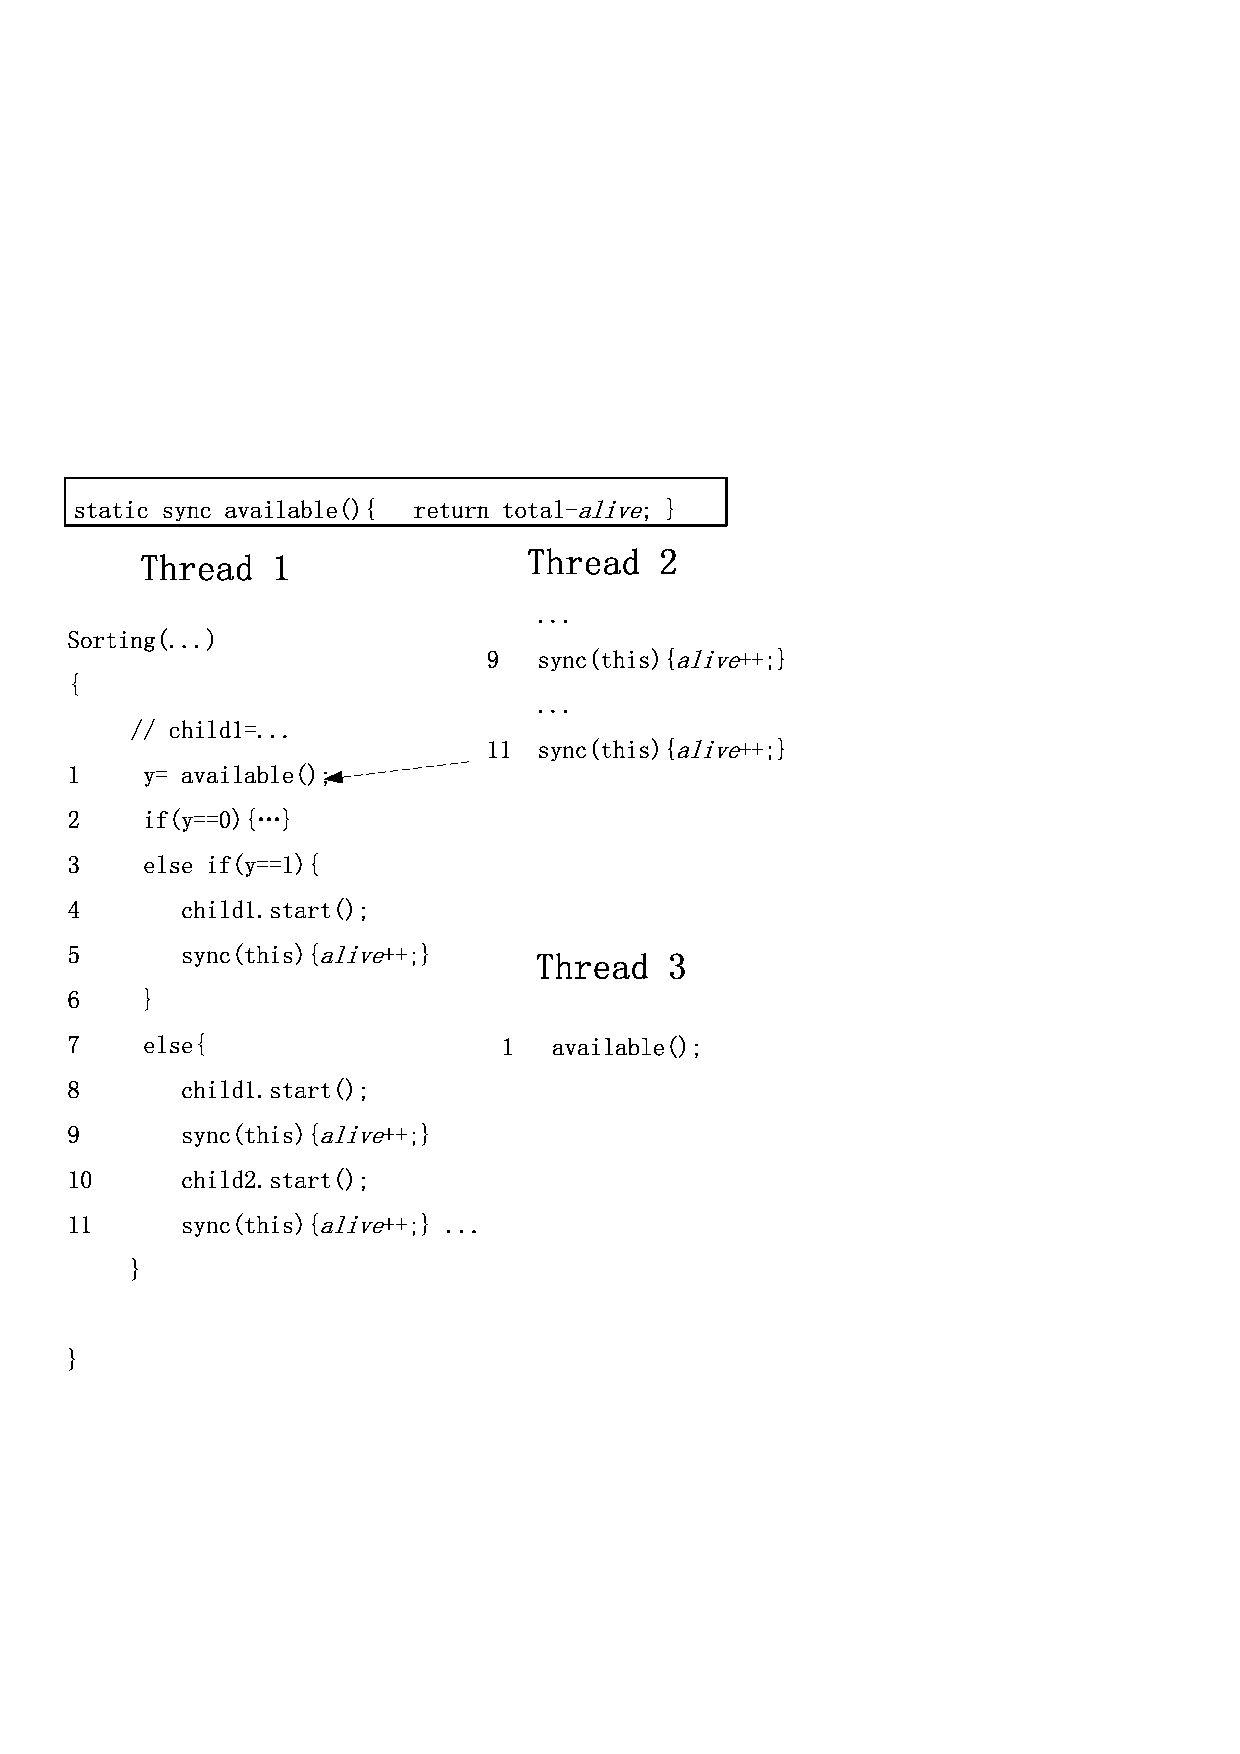
\includegraphics[scale=0.7]{cases/Visio-msort.pdf}
\caption{Relaxation of Paths}\label{fig:relax2}
\end{figure}


\section{Validity Threat}
Java method can have 65535 bytecode instructions maximally. Therefore, we count the number of bytecode instructions inside each method, if the number exceeds 65525, we avoid instrumenting the method. The consequence is that, we will miss the races inside the method. In this case, we specify the variables read from the method to be equal to their concrete values in the constraints. THe constraint solver can proceed safely without being affected by such methods.

We do not support the boolean operations such as $\&$, bit operators $<<$, which contributes to most of our misses.



